\documentclass{standalone}
\usepackage{tikz}
\usetikzlibrary{patterns, angles}

\begin{document}
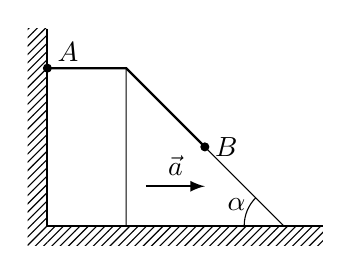
\begin{tikzpicture}
	\coordinate (A) at (0, 2);
    \coordinate (C) at (0, 2.5);
    \coordinate (O) at (0, 0);
    \coordinate (D) at (3.5, 0);
    \coordinate (E) at (3, 0);
    \coordinate (B) at (2, 1);
    \coordinate (F) at (1, 2);
       
	\draw [draw=none, pattern=north east lines] (C) rectangle (-0.25,-0.25);
	\draw [draw=none, pattern=north east lines] (0,-0.25) rectangle (D);	
	\draw [thick] (C) -- (O) -- (D);
	\draw [thick] (A) node [above=6pt, right] {$A$} -- (F) -- (B) node [above, right] {$B$};
	\draw  (F) -- (E) -- (1, 0) -- cycle;
	\draw [fill] (A) circle (0.05);	
	\draw [fill] (B) circle (0.05);
	\pic [draw, -, angle eccentricity=1.5] {angle = B--E--O};
	\node [left=17pt, above=2pt] at (E) {$\alpha$};
	\draw [arrows={-latex}, thick] (1.25, 0.5) -- (2, 0.5) node [above, midway] {$\vec{a}$};
\end{tikzpicture}
\end{document}